
\documentclass[a4paper]{article}

%% Language and font encodings
\usepackage[english]{babel}
\usepackage[utf8x]{inputenc}
\usepackage[T1]{fontenc}
\usepackage{verse}
\usepackage[noend]{algpseudocode}
\usepackage{listings}

%% Sets page size and margins
\usepackage[a4paper,top=3cm,bottom=2cm,left=3cm,right=3cm,marginparwidth=1.75cm]{geometry}

%% Useful packages
\usepackage{amsmath}
\usepackage{graphicx}
\usepackage[colorinlistoftodos]{todonotes}
\usepackage[colorlinks=true, allcolors=blue]{hyperref}

\usepackage[T1]{fontenc}

\newcommand{\verso}[1] {
\settowidth{\versewidth}{123456789012345678901234567890}%
\begin{minipage}[t]{\dimexpr\versewidth+1pt\relax}
\begin{verse}[\versewidth]
{\fontfamily{qzc}\selectfont\large
  #1
}
\end{verse}
\end{minipage}\bigskip
}



\title{Trabajo Práctico 3}
\author{}



\begin{document}
\maketitle

\section{Ayudando a los gorilas - Peso 8}
\subsection{Explicación}
En este problema nos piden que escribamos una algoritmo que nos permita decidir si en el nombre del gorila aparece un string que es resultado que quitarle un prefijo y un sufijo del mismo. Esto es equvalente a decir que el apodo es un substring del string original.\\
Dado que los nombres de los gorilas pueden ser muy largos, la complejidad esperada es de $O(N)$. Una aproximaci\'on trivial al problema seria ver si coincide el apodo con cada una uno de nombre, pero esto nos llevari\'ia a una algoritmo de complejidad temporal $O(NA)$, lo cual no es admisible. Nuestra propuesta nos llevar\'a a un algoritmo de complejidad $O(N+A)$, pero dado que $A < N$, ser\'a igual a $O(N)$. El algoritmo es conocido con el nombre de Algoritmo Z, y aprovecha informaci\'on de los sufijos anteriores que ya calculamos para calcular el actual.
El algoritmo Z, dado un string {\tt S}, nos devuelve un array (llamemoslo {\tt Z}) tal que {\tt Z[i]} es igual a la cantidad de caracteres en que coinciden {\tt S} y {\tt S[i:]} para $0 < i < |S|$. {\tt Z[0]} se suele obviar, ya que su valor es igual a la longitud del string.\\
Para aplicarlo en nuestro problema, lo que haremos ser\'a concatenar el apodo con el nombre y luego generar el array. Para saber si el apodo se encuentra en el nombre, bastara con buscar en las posiciones entre $A$ y $A+N$ si hay alg\'un valor mayor o igual a $A$, si lo hay significa que esa posici\'on del nombre (corrida $A$ lugares) coincide con la concatenaci\'on del apodo y el nombre en al menos $A$ lugares, y por como el apodo es prefijo de la misma, en $A$ lugares con este.\\
Pasemos a la explicaci\'on del algoritmo: El mismo usa tres indices, 
{\tt i} que es indice que estamos analizando en ese momento y {\tt r} y {\tt l} que son el indice del primer y ultimo caracter del substring que empieza antes de {\tt i} y termina lo m\'as a la derecha posible. \\
Veamos que pasa en cada momento cuando queremos calcular $Z[i]$.
Si $i>r$, significa que no existe ningun substring que sea prefijo de $S$, empiece antes de $i$ y termine despues de \'el. En este caso vamos leyendo los caracteres de $S$ a partir de $i$, hasta que dejen de coincidir con el inicio de S. Se actualizan $r$, $l$ y $Z[i]=l-r+1$.\\
Si $i\le r$, utilizaremos los resultados anteriores. Sea $j = i-l$, podemos ver que como $S[l]$ coincide con $S$ en $l-r+1$ caracteres, $S[i:]$ coincide en al menos $r-i+1$ caracteres con $S[j:]$ (que son los que se encuentran entre $l$ y $r$). Ahora se parte nuevamente en dos casos:\\
Si $Z[j] < r-i+1$ significa que $Z[i] = r-i+1$, ya que si fuera mayor, coincidiria en el caracter $S[r+1]$, pero entonces $S[j:]$ tambien lo haria, lo cual no puede pasar, porque si no $r$ podr\'ia haber seguido avanzando cuando $i$ habia tenido el valor de $j$. $Z[j] \le r-i+1$\\
Finalmente, si $Z[j] \geq r-i+1$ significa que coincidimos hasta $r$, as\'i que seguimos la comparacion a partir de aqu\'i

\subsection{Complejidad}
Para ver que nuestro algoritmo cumple con la complejidad esperada, tenemos que demostrar el algoritmo Z es $O(n)$ siendo $n$ la longitud del string\\
Si ignoramos los dos {\tt while} (Nos imaginamos que la condicion falla) est\'a claro que el algoritmo es Lineal, ya que es hacemos $n$ veces una cantidad que es $O(1)$ de operaciones.\\
Analicemos cuantas veces en total se ejecutan las operaciones dentro de los {\tt while}. Para eso usaremos la invariante mensionada antes: En cada paso del {\tt for}, \emph{r no se decrementa}.
Asi, como en cada operaci\'on del while, incrementamos $r$ en $1$, y $r$ est\'a acotada por $n$ las operaciones de los {\tt while} tambi\'en ser\'an $O(n)$ en total, dando la complejidad esperada.\\
Tenemos que tener un poco de cuidado con el {\tt r----} que hacemos despues de cada {\tt while} para que $r$ se encuentre en el \'ultimo caracter del prefijo. En el primero es facil de ver que r no decrementa, ya que $i>r$, y luego hacemos la asignaci\'on, con lo que $r$ es ahora mayor y, en el peor de los casos, no entra en el {\tt while} $r$ decrementar\'a en $1$, pero como ya se hab\'ia incrementado, ser\'a mayor o igual a su valor anterior.\\
En el segundo {\tt while} no podemos usar esto, pero como sabiamos que $r$ era el ultimo caracter que matcheaba, sabemos que entrar\'a la primera vez, y podemos considerar esta iteraci\'on entre las $O(1)$ operaciones del {\tt for} ya que este incremento se cancelar\'a con el decremento del final, as\'i todos las dem\'as iteraciones ser\'an incrementos efectivos.
Finalente el string que le pasamos a este algoritmo es de longitud $A+N$ y como $A \leq N$, es $O(N)$.
Luego iteramos sobre el resultado del algoritmo Z, lo que tambien tiene complejidad $O(N)$. \\
Dado que todas estas operaciones son $O(N)$, el algoritmo cumple con la cota del problema. 





\pagebreak
\section{Buscando a los alumnos - Peso 10}
\subsection{Explicación}

Para resolver este problema usamos la estructura de datos $trie$ vista en clase.
Primero leemos las direcciones y guardamos en el $trie$ los prefijos según lo indicado en el STDIN.
Para cada palabra p de longitud l, insertar en un trie tiene complejidad temporal O(l). Luego si tenemos $A$ direcciones, $D_{1},...,D_{A}$, cuya longitudes son $|D_{1}|,...,|D_{A}|$ respectivamente, el costo de insertar en el trie las $A$ direcciones es de O(S) siendo S la suma de las longitudes de las palabras, es decir $|D_{1}|+...+|D_{A}|$.\\

Modificamos levemente el clásico $trie$ agregando un contador que llamamos $count$, que cuenta las veces que se paso por un carácter durante la inserción de una nueva palabra.

\begin{lstlisting}[language=c++]
Trie
	map<char,Trie*> children;
	bool final;	
	int count;
\end{lstlisting}

Mientras insertamos una palabra vamos siguiendo un camino. Para contar las veces que se pasó por este camino, tenemos el contador que va sumando 1 cada vez que pasamos por un carácter.\\

Por ejemplo, si en un trie insertamos las palabras $hola$, $holamundo$, $mundo$, $mundial$ y $m$, en $count$ tendremos contadas las veces que pasamos por cada carácter de la siguiente manera:

\begin{center}
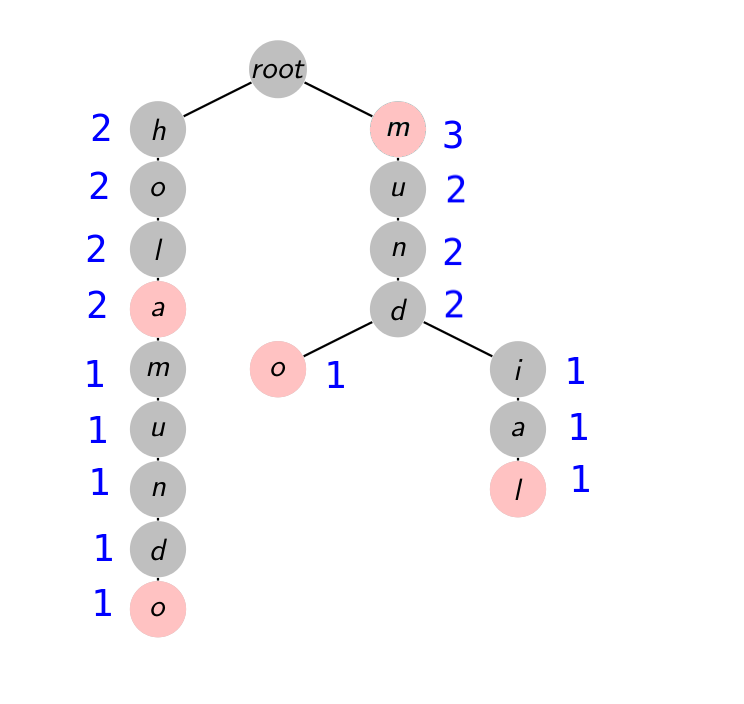
\includegraphics[width=8.5cm,height=6.5cm,keepaspectratio]{trieEjemplo.png}
\end{center}

Luego como en el trie guardamos los prefijos y lo que interesa saber es la cantidad de prefijos compartidos, viendo el valor de $count$ asociado a cada prefijo, podremos saber cuántos otros prefijos incluyen al prefijo en cuestión. De esta manera, vamos a poder responder a lo sumo cuantas direcciones comparten este prefijo, y esto lo hacemos viendo el máximo valor alcanzado de la variable $count$ asociado a los prefijos.\\

Como lo que interesa saber es el mínimo valor T que cumple que para cada dirección de correo electrónico junto con su prefijo, existen a lo sumo T direcciones que comparten ese prefijo, tenemos que buscar en el trie cuál es el valor máximo que alcanza la variable $count$ asociada a los prefijos.\\
Por lo tanto, a fin de consultar el valor $count$ asociado a cada prefijo, tendremos que buscar cada prefijo en el trie y devolver el valor $count$.\\
\newpage

\subsection{Complejidad}
La complejidad temporal de leer cada palabra del STDIN e insertarla en el trie, tiene un costo de O(S+S'), donde S es la suma de las longitudes de las direcciones y S' es la suma de las longitudes de los prefijos. Como S' $\leq$ S, el siguiente FOR tiene complejidad temporal O(S).\\

\begin{lstlisting}[language=c++]
	for(int i=0; i<n; i++) {
		cin >> address >> prefixSize;
		prefixes[i] = address.substr(0,prefixSize);
	}
    
\end{lstlisting}
\

Dado un prefijo $D_{i}$, buscar en el trie tiene una complejidad temporal $O(|D_{i}|)$, donde $|D_{i}|$ es la longitud de la palabra $D_{i}$.\\
Luego, la complejidad de buscar cada prefijo $D'_{i}$ en el trie es de 
O(S'), siendo S' la suma de las longitudes de los prefijos, es decir $|D'_{1}|+...+|D'_{A}|$.\\
Luego saber el máximo count de entre todos los prefijos tiene un costo temporal de O(S'), correspondiente a buscar cada prefijo y acceder a count asociado.\\
Por lo tanto, la complejidad temporal total es O(S + S') = O(S), donde S es la longitud de las direcciones y S' es la longitud de los prefijos.

\newpage

\pagebreak
\section{Ciencia Argentina - Peso 7}
\subsection{Modelado}

Este problema puede ser resuelto con una tabla aditiva, ya que contamos con el operador asociativo suma y podemos aprovechar que este operador tiene inverso (la resta) para poder hacer consultas de prefijos. En este caso, vamos a necesitar un vector acumulado V bidimensional de $(C+1)x(A+1)$ elementos, ya que contamos con una matriz de entrada $M = CxA$, donde C son las categorías y A las antigüedades. Luego, bastará con realizar queries en V para obtener la suma de los montos $M_{i,j}$ que son parte del sueldo de un docente con cargo c2 y antiguedad a2 , y que no pueden cobrar docentes con cargo c1 o antiguedad a1, con $c1 \leq i \leq c2$ y $a1 \leq j \leq a2$.


\subsection{Demostración}
Cada elemento de V estará dado por la siguiente sumatoria:\\
\begin{center}
$V_{i,j} = \sum_{c=0}^{i-1}\sum_{a=0}^{j-1} M_{c,a} $
\end{center}


Utilizando programación dinámica podemos construir V en tiempo lineal de la siguiente forma: \\
\begin{center}
$V_{0,j} = V_{i,0} = 0,  \forall i,j$  con  $0 \leq i \leq C, 0 \leq j \leq A$
\end{center}

\begin{center}
$V_{i+1,j+1} = M_{i,j} + V_{i,j+1} + V_{i+1, j} - V_{i,j},   \forall i,j$  con  $0 \leq i < C, 0 \leq j < A$
\end{center}

Viendo el código a continuación, podemos ver que este vector bidimensional V se construye con un for loop que itera las categorías y otro las antiguedades, teniendo un costo de $O(AC)$.

\begin{lstlisting}[language=c++]

    for (int i=1; i<=C;i++){
      for(int j=1;j<=A;j++){
        // no hace falta guardar la matrix M, 
        // directamente uso el input para armar V
        cin >> v_ij; 
        V[i][j] = v_ij + V[i-1][j] + V[i][j-1] - V[i-1][j-1];
      }
    }

\end{lstlisting}
Luego podremos realizar las queries de rangos dados c1,c2 categorías y a1,a2 antigüedades:

\begin{center}
$Q(c1 , a1 , c2 , a2 ) = \sum_{i=c1}^{c2-1}\sum_{j=a1}^{a2-1} M_{i,j} $
\end{center}

utilizando directamente el vector V y calculando 4 valores únicamente en tiempo constante:

\begin{center}
$Q(c1 , a1 , c2 , a2 ) = V_{c2,a2} - V_{c1,a2} - V_{c2,a1} + V_{c1,a1} $
\end{center}

De esta forma, si tenemos Q queries, tenemos una complejidad total de $O(AC +Q)$



\pagebreak
\section{Diversión asegurada - Peso 12}
\verso{ % 1 1
Aunque vagos hayan estado,\\
Y no hayan hecho poemas,\\
deben ser recompensados,\\
por hacernos los problemas.\\
}
\verso{ % 2 1
Y por qué no vacaciones,\\
Creo que se las merecen,\\
calculemos las diversiones,\\
un poco antes de que empiecen.\\
}
\verso{ % 3 1
Si va a haber varios eventos,\\
a lo ancho y a lo largo,\\
debemos estar atentos,\\
a no terminar amargos.\\
}
\verso{ % 4 1
Tenemos de los sucesos,\\
cuánta risa nos producen,\\
queremos saber de esos,\\
qué dos mayor suma inducen.\\
}
\verso{ % 1 2
Hacer que el programa mande,\\
de una manera eficiente,\\
en un rango, el más grande,\\
lo dijo Agustín, no miente.\\
}
\verso{ % 2 2
Supongamos que asistimos,\\
en un rango que nos dieron,\\
al hecho más divertido,\\
no me alcanza, otro quiero.\\
}
\verso{ % 3 2
El más gracioso es la brecha,\\
que al rango en dos me segmente.\\
A la izquierda y la derecha,\\
me quedan fiestas con gente.\\
}
\verso{ % 4 2
Pero esto es fácil, repito,\\
encontramos los mejores,\\
de cada intervalito,\\
para que de risa llores.\\
}
\verso{ % 1 3
Y ahora al más grande de ambos,\\
lo sumamos al primero,\\
la respuesta ya encontramos,\\
con sólo un poco de esmero.\\
}
\verso{ % 2 3
Si en la complejidad pensamos,\\
implementamos un segment tree,\\
solo que en cada intervalo,\\
hay que multiplicar por three.\\
}
\verso{ % 3 3
Espero no decepcione\\
el poema, es que me dormía,\\
la próxima una canción, eh,\\
hablando de geometría.\\
}

\subsection{Modelado y Explicación}

Para resolver este problema usaré una adaptación de RMQ (en este caso, será Range Maximum Query). Podemos pensar que "cuán divertido es un evento" es el número que guardaremos en las hojas del segment tree, luego completamos los nodos con la operación "max", y ahora lo que queremos es básicamente los dos elementos más grandes del rango pedido (y después sumarlos).\\
¿Cómo vamos a encontrar los dos más grandes de un rango? Primero, de una manera tradicional encontramos el máximo del rango. En realidad, lo que vamos a guardar será el índice (es decir, el día) del evento más divertido (llamémoslo $E$). Ahora simplemente lo que queremos es el evento más divertido del rango, descartando E. Podemos pensar que el evento $E$ nos divide al rango en dos, los eventos que ocurren antes de E y los que ocurren después de E (alguno de estos conjunto puede ser vacío, pero no ambos pues todos los rangos toman por lo menos dos días distintos, ya que $U-P>=2$).\\
Entonces simplemente buscamos el más divertido de los eventos de antes y el más divertido de los de después de E, y comparamos esos dos. El más divertido de esos dos será en efecto el segundo más divertido de todo el rango dado. Sumamos este valor con el valor de E y obtenemos la diversión del rango.

\subsection{Demostración de complejidad}

Primero, en $O(D)$ ingresamos los valores de las diversiones de los eventos y los guardamos en un vector.
\\
Luego, completamos el vector "eventos" con números $0$ (que es el valor neutro de la función "max", pues todos los valores son no negativos). Para esto debemos calcular la mínima potencia de 2 más grande que D, que lo hacemos en O(log D), y luego completar el vector, que, como la potencia de 2 encontrada es a lo sumo D-1, completar lo hacemos en O(D).
\\
\begin{lstlisting}[language=c++]
int minPot2Mayor=1;
while(minPot2Mayor<D){
	minPot2Mayor*=2;
}
forn(i, minPot2Mayor-D){
	eventos.pb(0);
}
\end{lstlisting}

Luego, creamos el segment tree llamando a la función build pasándole el tamaño del vector, que es la mínima potencia de 2 encontrada, i.e. $O(2.D) = O(D)$. Esta funcion primero setea las hojas en el valor del evento correspondiente (del evento, no de su diversión):
\begin{lstlisting}[language=c++]
forsn(i, n, 2*n){
	stree[i]=i-n;
}
\end{lstlisting}
Como se ve, esto es $O(n) = O(D)$.

Y luego, va creando, de abajo para arriba, los nodos del segment tree, guardando el día del evento más divertido entre los eventos que indican sus hijos:
\begin{lstlisting}[language=c++]
for(int i=n-1; i>=1; i--){
	if(eventos[stree[2*i]]>eventos[stree[2*i+1]]){
		stree[i]=stree[2*i];
	}else{
		stree[i]=stree[2*i+1];
	}
}
\end{lstlisting}
Esto también tiene complejidad $O(n) = O(D)$

Hasta acá entonces armamos el segment tree con una complejidad $O(D)$, donde cada nodo indica el día del evento más divertido del rango que cubre.\\

Luego, falta responder las queries. Veamos lo que hace el programa en cada query cada query (adentro del while(R--)):\\
\\
1) Encontramos la posición del evento (llamado $E$) más divertido del rango: \\
\textbf{int posicionDeMaximo=ans(1, 0, eventos.size(), P, U)};\\
2) Encontramos la posición del evento más divertido a la izquierda de $E$: \\
\textbf{int posIzq=ans(1, 0, eventos.size(), P, posicionDeMaximo);}\\
3) Encontramos la posición para el más divertido a la derecha de $E$: \\
\textbf{int posDer=ans(1, 0, eventos.size(), posicionDeMaximo+1, U)};\\
\\
Finalmente, encontramos el más grande de los dos últimos eventos hallados, y lo sumamos al primero, en $O(1)$.\\
Al principio no se me había ocurrido un "elemento neutro" para la operación de buscar el índice, y contemplaba esos cosas con un $-1$. Pero escribiendo el informe me avivé de usar un índice neutro que contenga el elemento neutro, entonces en la función \textbf{ans}, si el rango del nodo en cuestión y el rango preguntado no se intersecan, devuelvo \textbf{INDICE\_NEUTRO}, día inventado por mí conteniendo un evento de diversión $0$ (ya que $0$ es el elemento neutro de la operación "max" en este caso, como ya vimos).
Esto se asigna acá:
\begin{lstlisting}[language=c++]
INDICE_NEUTRO = eventos.size();
eventos.pb(0);
\end{lstlisting}

Entonces la complejidad de responder una query es $3$ veces la complejidad de \textbf{ans} . La complejidad de \textbf{ans} es $O(log D)$, por lo visto en la clase de Agustín.
Luego, la complejidad de encontrar la respuesta para cada query es $O(3.log(D)) = O(log(D))$.\\

Finalmente, la complejidad de todo el algoritmo es $O(D + R.log(D))$, como se pide.

\newpage

\section{C\'odigo}

\subsection{Problema A}

\begin{lstlisting}[language=c++]
#include <bits/stdc++.h>

using namespace std;

string apodo, nombre;
vector<int> z;

void doz(string s){
    int n = (int)s.length();
    z = vector<int>(n, 0);
    
    int l, r;
    l = r = 0;
    for (int i=1; i<n; i++) {
        // Si i > r checkeamos normalmente
        if(i>r){
        
            l = r = i; //actualizo los valores
            while (r<n && s[r-l] == s[r])
                r++;
            r--; //ya no coincide, corrijo
            z[i] = r-l+1;
        
        } else {
        
            int j = i-l;

            if (z[j] < r-i+1) {
                z[i] = z[j];
            } else {
                // checkeamos a partir de r
                l = i; //como r va a aumentar, l ahora va a ser i
                while (r<n && s[r-l] == s[r])
                    r++;
                r--; //corrijo
                z[i] = r-l+1;
            }
        }
    }
}


int main(){
    cin >> nombre;
    cin >> apodo;
    doz(apodo+nombre);
    for(size_t i = apodo.length(); i < z.size(); i++){
        if(z[i]>= (int)apodo.length()){
            cout << "S" << endl;
            return 0;
        }
    }
    cout << "N" << endl;
}

\end{lstlisting}
\newpage
\subsection{Problema B}
\begin{lstlisting}[language=c++]
#include <bits/stdc++.h>

using namespace std;

class Trie{
	map<char,Trie*> children;
	bool final;	
	int count;
public:
	Trie() {
		children.clear();
		final = false;
		count = 0;
	}
	
	Trie(string &s, int pos) {
		count = 1;
		children.clear();
		if(pos == s.size()) {
			final = true;
			return;
		}
		final = false;
		children[s[pos]] = new Trie(s,pos+1);
	}
	
	void insert(string &s, int pos = 0) {
		count++;
		if(pos == s.size()) {
			final = true;
		} else if(children.find(s[pos]) == children.end()) {
			children[s[pos]] = new Trie(s,pos+1);
		} else {
			children[s[pos]]->insert(s,pos+1);
		}
		return;
	}
	
	int countPrefixes(string &s, int pos = 0){
		if(pos == s.size()) {
			return count;
		} else if(children.find(s[pos]) == children.end()) {
			return 0;
		} else {
			return children[s[pos]]->countPrefixes(s,pos+1);
		}
	}
};

int main() {
	int n;
	cin >> n;
	Trie addresses;
	string address;
	string prefixes[n];
	int prefixSize;
	int maxValue = 0;
	for(int i=0; i<n; i++) {
		cin >> address >> prefixSize;
		prefixes[i] = address.substr(0,prefixSize);
	}
	
	for(int i=0; i < n; i++){
		addresses.insert(prefixes[i]);
	}
	
	for(int i=0; i < n; i++){
		int count = addresses.countPrefixes(prefixes[i]);
		maxValue = max(maxValue, count);
	}
	
	cout << maxValue << endl;
}

\end{lstlisting}
\newpage
\subsection{Problema C}
\begin{lstlisting}[language=c++]

#include "iostream"
#include <cstring>
using namespace std;

int main()
{
    int C, A, Q;
    cin >> C;
    cin >> A;
    cin >> Q;
    // Creo arreglo acumulado V
    int V[C+1][A+1];
    memset(V,0,sizeof(V));
    int v_ij;
    // Lleno arreglo acum
    for (int i=1; i<=C;i++){
      for(int j=1;j<=A;j++){
        cin >> v_ij;
        V[i][j] = v_ij + V[i-1][j] + V[i][j-1] - V[i-1][j-1];
      }
    }

    // Ingreso queries
    int c1,a1,c2,a2;
    int answer = 0;
    for (int i=0;i<Q;i++){
      cin >> c1;
      cin >> a1;
      cin >> c2;
      cin >> a2;
      answer = V[c2][a2] - V[c1][a2] - V[c2][a1] + V[c1][a1];
      cout << answer << endl;
    }
    return 0;
}





\end{lstlisting}
\newpage
\subsection{Problema D}
\begin{lstlisting}[language=c++]

#include<iostream>
#include<math.h>
#include<algorithm>
#include<vector>

using namespace std;

#define forn(i,n) for(int i=0;i<(int)(n); i++)
#define forsn(i,s,n) for(int i=(s);i<(int)(n); i++)
#define pb push_back

typedef long long tint;

vector<int> stree;
vector<tint> eventos;
int INDICE_NEUTRO;

void build(int n){
	forn(i, 2*n){
		stree.pb(0);
	}
	forsn(i, n, 2*n){
		stree[i]=i-n;
	}
	for(int i=n-1; i>=1; i--){
		if(eventos[stree[2*i]]>eventos[stree[2*i+1]]){
			stree[i]=stree[2*i];
		}else{
			stree[i]=stree[2*i+1];
		}
	}
}

int ans(int node, int l, int r, int i, int j){
	if(i<=l && j>=r) {
		return stree[node];
	}
	if(l>=j || r<=i) {
		return INDICE_NEUTRO;
	}
	int ind1=ans(2*node, l, (l+r)/2, i, j);
	int ind2=ans(2*node+1, (l+r)/2, r, i, j);
	if(eventos[ind1]>eventos[ind2]){
		return ind1;
	}else{
		return ind2;
	}
}

int main (){
	int D, R;
	cin>>D>>R;
	forn(i, D){
		tint e; cin>>e;
		eventos.pb(e);
	}
	int minPot2Mayor=1;
	while(minPot2Mayor<D){
		minPot2Mayor*=2;
	}
	forn(i, minPot2Mayor-D){
		eventos.pb(0);
	}
	build(eventos.size());
	INDICE_NEUTRO = eventos.size();
	eventos.pb(0);
	while(R--){
		int P, U;
		cin>>P>>U;
		int posicionDeMaximo=ans(1, 0, eventos.size(), P, U);
		int posIzq=ans(1, 0, eventos.size(), P, posicionDeMaximo);
		int posDer=ans(1, 0, eventos.size(), posicionDeMaximo+1, U);
		tint segundoMayor=max( eventos[posIzq], eventos[posDer] );
		cout<< eventos[posicionDeMaximo]+segundoMayor <<endl;
	}
}



\end{lstlisting}


\end{document}